% PHU LUC - bo cuc va thong tin theo AI_PROJECT, co bo sung noi dung mau cua thay.
\clearpage
\pagestyle{plain}
\setcounter{table}{0}\renewcommand{\thetable}{PL.\arabic{table}}
\section*{PHỤ LỤC A. HÌNH ẢNH}
\phantomsection\addcontentsline{toc}{section}{PHỤ LỤC A. HÌNH ẢNH}
\setcounter{figure}{0}\renewcommand{\thefigure}{A.\arabic{figure}}
\printappendixfigures
\clearpage
\subsection*{A.1. Thiết kế giao diện Admin}
Hình~\ref{fig:app-admin-design} minh họa hai nhóm nội dung kiểm duyệt phòng và quản lý tài khoản. Thẻ thông tin đặt thao tác chấp thuận, từ chối hoặc quản lý trạng thái cạnh đối tượng cần xử lý. Phần tổng quan và bộ lọc hỗ trợ xác định nhóm hồ sơ trước khi mở chi tiết; số liệu trong hình là dữ liệu minh họa thiết kế.
\begin{figure}[H]\centering
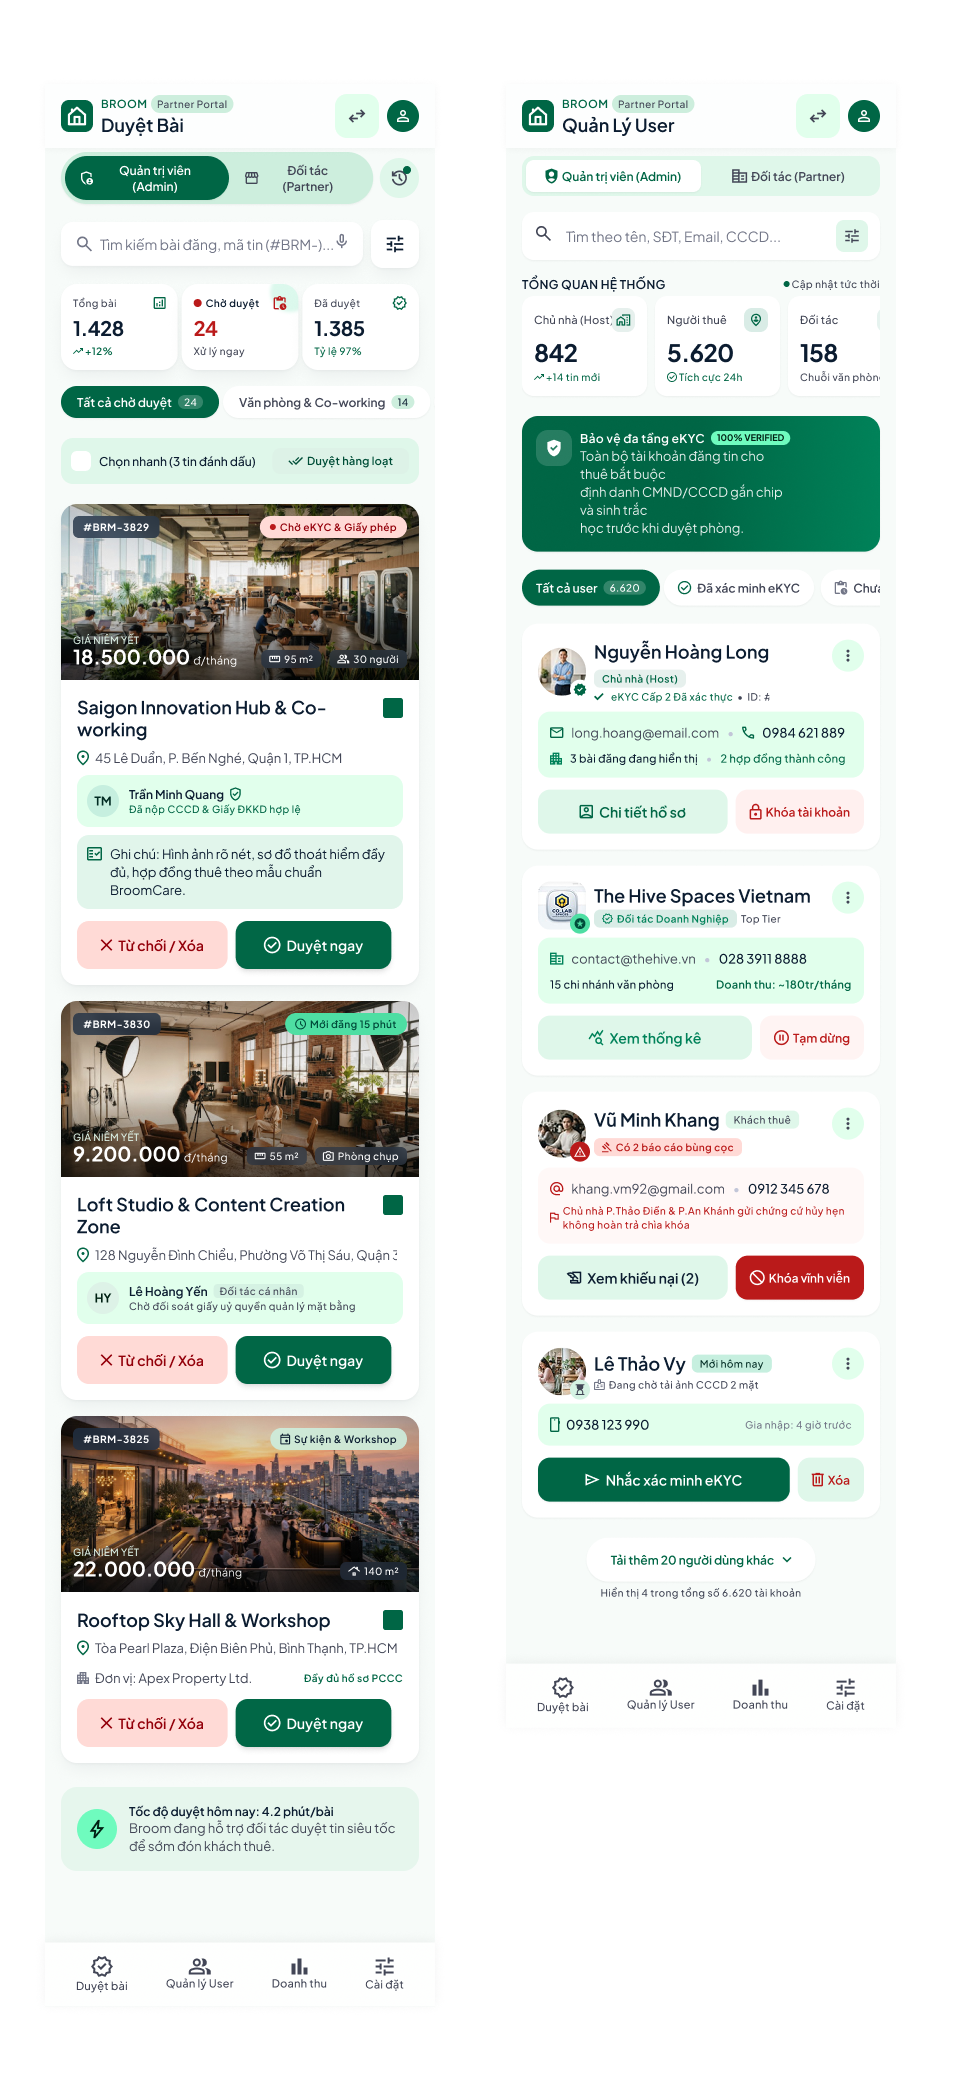
\includegraphics[width=\textwidth,height=0.76\textheight,keepaspectratio]{chapter3/admin-design.png}
\caption{Phương án thiết kế kiểm duyệt và quản lý trong phân hệ Admin.}\label{fig:app-admin-design}
\end{figure}

\clearpage


\clearpage
\section*{PHỤ LỤC B. TRUY VẤN SQL VÀ TRUY VẤN FIRESTORE}
\phantomsection\addcontentsline{toc}{section}{PHỤ LỤC B. TRUY VẤN SQL VÀ FIRESTORE}
\appendixnote{Phụ lục minh họa các thao tác truy vấn dữ liệu trong BroomSharing. Vì kiến trúc sử dụng Cloud Firestore (NoSQL), các câu SQL chỉ biểu diễn logic tương đương, không phải mã có thể thực thi trực tiếp trên Firestore.}
\subsection*{B.1. Liệt kê không gian đang được công bố}
\begin{minted}{sql}
-- Pseudo-SQL: minh hoa truy van tuong duong
SELECT space_id, title, address, price, status
FROM spaces
WHERE status = 'available'
ORDER BY created_at DESC;
\end{minted}
\noindent\textbf{Lệnh Java/Firestore tương ứng (minh họa):}
\begin{minted}{java}
FirebaseFirestore db = FirebaseFirestore.getInstance();
db.collection("spaces")
  .whereEqualTo("status", "available")
  .orderBy("createdAt", Query.Direction.DESCENDING)
  .get()
  .addOnSuccessListener(result -> {
      // Anh xa document sang Model Space
  });
\end{minted}
\noindent\textit{Lưu ý:} tổ hợp lọc và sắp xếp có thể đòi hỏi tạo composite index trên Firestore theo hướng dẫn của Firebase.

\subsection*{B.2. Tìm kiếm không gian theo mức giá}
\begin{minted}{sql}
-- Pseudo-SQL: minh hoa logic loc theo muc gia
SELECT space_id, title, price
FROM spaces
WHERE status = 'available'
  AND price BETWEEN :min_price AND :max_price
ORDER BY price ASC;
\end{minted}
\noindent\textbf{Hướng truy vấn Firestore:} dùng \texttt{whereGreaterThanOrEqualTo}, \texttt{whereLessThanOrEqualTo} và \texttt{orderBy} trên trường giá. Trước khi triển khai phải thống nhất đơn vị tiền tệ và kỳ thuê để dữ liệu có thể so sánh được.

\Needspace{9\baselineskip}
\subsection*{B.3. Danh sách booking của một người dùng}
\begin{minted}{sql}
-- Pseudo-SQL: minh hoa logic truy van
SELECT booking_id, space_id, start_time, end_time, status
FROM bookings
WHERE renter_id = :current_user_id
ORDER BY created_at DESC;
\end{minted}
\noindent\textbf{Hướng truy vấn Firestore:} lọc theo \texttt{renterId} của người dùng hiện tại, sau đó sắp xếp theo \texttt{createdAt}; quy tắc Security Rules phải kiểm tra quyền đọc của tài khoản. Thao tác đặt trùng thời gian cần được xử lý nhất quán và không chỉ dựa vào kiểm tra ở giao diện \parencite{firebase_security,firebase_transaction}.

\subsection*{B.4. Liệt kê không gian do một chủ sở hữu quản lý}
\begin{minted}{sql}
-- Pseudo-SQL: danh sach tin dang cua Owner
SELECT space_id, title, price, status, created_at
FROM spaces
WHERE owner_id = :current_owner_id
ORDER BY created_at DESC;
\end{minted}
\noindent\textbf{Hướng truy vấn Firestore:} sử dụng điều kiện lọc \texttt{ownerId} theo định danh đăng nhập và sắp xếp \texttt{createdAt}. Quyền sửa tin cần được kiểm tra bằng Security Rules thay vì chỉ kiểm soát nút trên giao diện \parencite{firebase_security}.

\subsection*{B.5. Cập nhật trạng thái yêu cầu đặt thuê}
\begin{minted}{sql}
-- Pseudo-SQL: Owner xu ly yeu cau booking
UPDATE bookings
SET status = 'approved', updated_at = :now
WHERE booking_id = :booking_id
  AND status = 'pending'
  AND owner_id = :current_owner_id;
\end{minted}
\noindent\textbf{Hướng xử lý Firestore:} trước khi chuyển trạng thái, xác nhận quyền của chủ không gian và trạng thái hiện tại; nếu có dữ liệu phụ thuộc hoặc điều kiện cạnh tranh, xét cơ chế transaction và kiểm tra tính nhất quán \parencite{firebase_transaction,firebase_security}. Câu truy vấn trên chỉ dùng để giải thích điều kiện nghiệp vụ.

\clearpage
\section*{PHỤ LỤC C. DANH MỤC BẢNG, BIỂU}
\phantomsection\addcontentsline{toc}{section}{PHỤ LỤC C. DANH MỤC BẢNG, BIỂU}
\appendixnote{Danh mục bảng biểu trong phần thân báo cáo được sinh tự động; số trang và số thứ tự sẽ cập nhật theo kết quả biên dịch cuối cùng.}
\printappendixtables

\clearpage
\section*{PHỤ LỤC D. ĐƯỜNG DẪN TÀI NGUYÊN ĐỒ ÁN}
\phantomsection\addcontentsline{toc}{section}{PHỤ LỤC D. ĐƯỜNG DẪN TÀI NGUYÊN ĐỒ ÁN}
\appendixnote{Các tài nguyên trực tuyến hỗ trợ theo dõi tiến độ, đối chiếu mã nguồn và kiểm tra minh chứng thực hiện của nhóm.}

\subsection*{Bảng phân công nhiệm vụ}
Bảng phân công được nhóm lưu trực tuyến để giảng viên theo dõi nhiệm vụ, tiến độ và kết quả của từng thành viên.
\begin{center}
{\Large\bfseries
\ifdefempty{\BroomSheetURL}{\faFileExcel\ XEM BẢNG PHÂN CÔNG CÔNG VIỆC}{\href{\BroomSheetURL}{\faFileExcel\ XEM BẢNG PHÂN CÔNG CÔNG VIỆC}}
}
\end{center}

\subsection*{Link đồ án -- GitHub}
Mã nguồn BroomSharing được quản lý bằng GitHub nhằm phục vụ việc xem xét các thành phần dự án và lịch sử phát triển.
\begin{center}
{\Large\bfseries
\ifdefempty{\BroomGitHubURL}{\faGithub\ XEM SOURCE CODE BROOMSHARING}{\href{\BroomGitHubURL}{\faGithub\ XEM SOURCE CODE BROOMSHARING}}
}
\end{center}

\subsection*{Đường dẫn học phần}
Các tài liệu và yêu cầu được giảng viên công bố là cơ sở để đối chiếu cấu trúc và tiêu chí đánh giá đồ án.
\begin{center}
{\large\bfseries
\ifdefempty{\BroomCourseURL}{\faGraduationCap\ XEM THÔNG TIN HỌC PHẦN}{\href{\BroomCourseURL}{\faGraduationCap\ XEM THÔNG TIN HỌC PHẦN}}
}
\end{center}

\subsection*{GitHub Projects và thư mục minh chứng}
Bảng công việc và tập ảnh ghi nhận tiến độ được quản lý độc lập với báo cáo để thuận tiện cập nhật.
\begin{center}
{\large\bfseries
\ifdefempty{\BroomProjectsURL}{\faTasks\ XEM NHẬT KÝ PHÂN CÔNG}{\href{\BroomProjectsURL}{\faTasks\ XEM NHẬT KÝ PHÂN CÔNG}}
}\par\smallskip
{\large\bfseries
\ifdefempty{\BroomImagesURL}{\faImages\ XEM THƯ MỤC ẢNH MINH CHỨNG}{\href{\BroomImagesURL}{\faImages\ XEM THƯ MỤC ẢNH MINH CHỨNG}}
}
\end{center}


\clearpage
\section*{PHỤ LỤC E. BẢNG PHÂN CÔNG VÀ MINH CHỨNG NHÓM}
\phantomsection\addcontentsline{toc}{section}{PHỤ LỤC E. BẢNG PHÂN CÔNG VÀ MINH CHỨNG NHÓM}
\appendixnote{Bảng phân công nêu trách nhiệm và sản phẩm bàn giao của từng thành viên; minh chứng cần đối chiếu được với GitHub Projects, Google Sheets hoặc lịch sử commit.}
\begin{longtable}{@{}>{\raggedright\arraybackslash}p{4.2cm}p{6.7cm}p{3.2cm}@{}}\caption{Bảng nhiệm vụ nhóm cần xác nhận}\label{tab:append_assign}\\\toprule
\textbf{Thành viên}&\textbf{Nhiệm vụ riêng}&\textbf{Commit / Issues / Sheet}\\\midrule\endfirsthead
\toprule\textbf{Thành viên}&\textbf{Nhiệm vụ riêng}&\textbf{Commit / Issues / Sheet}\\\midrule\endhead
Lữ Võ Hoàng Phúc& Bổ sung phần việc thực tế theo log triển khai BroomSharing.& Chưa cung cấp\\
Lâm Hoàng& Ghi đúng hạng mục đã nhận và kết quả bàn giao.& Chưa cung cấp\\
Từ Trương Thanh Trúc& Ghi đúng hạng mục đã nhận và kết quả bàn giao.& Chưa cung cấp\\
\bottomrule\end{longtable}
\noindent\textbf{Minh chứng nên kèm:} ảnh phân công GitHub Projects hoặc Google Sheets; ảnh lịch sử commit thể hiện tên người thực hiện, thời gian và tệp thay đổi; liên kết commit tương ứng. Không suy đoán kết quả của từng thành viên khi chưa có dữ liệu.

\clearpage
\section*{PHỤ LỤC F. TƯ LIỆU VÀ KIỂM TRA BỔ SUNG}
\phantomsection\addcontentsline{toc}{section}{PHỤ LỤC F. TƯ LIỆU VÀ KIỂM TRA BỔ SUNG}
\appendixnote{Các tài liệu vượt khỏi dung lượng báo cáo chính hoặc minh chứng phát sinh trong quá trình triển khai được đặt tại đây để không làm gián đoạn dòng trình bày của bảy chương.}
\begin{enumerate}[leftmargin=*]
\item Nhật ký thử nghiệm trên emulator và thiết bị thực: phiên bản Android, loại thiết bị, thao tác thực hiện, kết quả, ảnh/log.
\item Trích xuất cấu trúc collection/document Firestore và Security Rules đã kiểm tra; không công khai khóa bí mật.
\item Ảnh chụp bổ sung về màn hình tìm kiếm, hồ sơ, chủ không gian, xử lý booking, bản đồ hoặc QR (chỉ khi đã thực hiện).
\item Các đoạn truy vấn hoặc mã Java/Repository quá dài: chuyển sang mã nguồn GitHub và liên kết đến dòng code tương ứng.
\item Kịch bản kiểm thử bổ sung, lỗi đã phát hiện và cách khắc phục; ghi tách biệt với chức năng chỉ mới được đề xuất.
\end{enumerate}

\clearpage
\section*{PHỤ LỤC G. PHÂN RÃ CHỨC NĂNG CHI TIẾT}
\phantomsection\addcontentsline{toc}{section}{PHỤ LỤC G. PHÂN RÃ CHỨC NĂNG CHI TIẾT}
\label{app:chapter2-details}
\setcounter{figure}{0}\renewcommand{\thefigure}{G.\arabic{figure}}
Các nhóm chức năng dưới đây triển khai chi tiết từ sơ đồ tổng quát ở Chương 2. Mỗi nhóm gắn với một phạm vi nghiệp vụ; các bước dùng chung được giữ trong cùng nhóm để thể hiện trách nhiệm xử lý.

\clearpage
Nhóm tài khoản quản lý đăng nhập, đăng ký, khôi phục mật khẩu và phiên truy cập theo vai trò.
\begin{figure}[H]\centering
\includegraphics[page=2,width=\textwidth,height=0.78\textheight,keepaspectratio]{chapter2/usecase_decomposition_v2.pdf}
\caption{Phân rã chức năng: tài khoản và phiên.}\label{fig:app-functions-2}
\end{figure}

\clearpage
Khám phá không gian kết hợp tìm kiếm, bộ lọc, bản đồ và thông tin phòng trước khi đặt.
\begin{figure}[H]\centering
\includegraphics[page=3,width=\textwidth,height=0.78\textheight,keepaspectratio]{chapter2/usecase_decomposition_v2.pdf}
\caption{Phân rã chức năng: khám phá không gian.}\label{fig:app-functions-3}
\end{figure}

\clearpage
Yêu cầu đặt chỗ bao gồm chọn kỳ thuê, kiểm tra khả dụng, chốt giá và mở QR với thời hạn giữ lịch tạm.
\begin{figure}[H]\centering
\includegraphics[page=4,width=\textwidth,height=0.78\textheight,keepaspectratio]{chapter2/usecase_decomposition_v2.pdf}
\caption{Phân rã chức năng: tạo yêu cầu đặt chỗ.}\label{fig:app-functions-4}
\end{figure}

\clearpage
Theo dõi lượt thuê phân biệt lịch sử, thời hạn thanh toán và điều kiện hủy; nhả lịch đi cùng cập nhật trạng thái.
\begin{figure}[H]\centering
\includegraphics[page=5,width=\textwidth,height=0.78\textheight,keepaspectratio]{chapter2/usecase_decomposition_v2.pdf}
\caption{Phân rã chức năng: lịch đặt và hủy.}\label{fig:app-functions-5}
\end{figure}

\clearpage
Hồ sơ Host được xét duyệt riêng với minh chứng vị trí hoặc hình ảnh của tài sản.
\begin{figure}[H]\centering
\includegraphics[page=6,width=\textwidth,height=0.78\textheight,keepaspectratio]{chapter2/usecase_decomposition_v2.pdf}
\caption{Phân rã chức năng: hồ sơ host và xác minh.}\label{fig:app-functions-6}
\end{figure}

\clearpage
Quản lý tài sản tách tòa nhà, phòng, cấu hình giá và lịch; công bố phòng phụ thuộc trạng thái xét duyệt và hoạt động.
\begin{figure}[H]\centering
\includegraphics[page=7,width=\textwidth,height=0.78\textheight,keepaspectratio]{chapter2/usecase_decomposition_v2.pdf}
\caption{Phân rã chức năng: quản lý không gian.}\label{fig:app-functions-7}
\end{figure}

\clearpage
Vận hành lượt thuê phân biệt nhận phòng, hoàn tất và không đến, không suy ra đã sử dụng chỉ từ thời gian.
\begin{figure}[H]\centering
\includegraphics[page=8,width=\textwidth,height=0.78\textheight,keepaspectratio]{chapter2/usecase_decomposition_v2.pdf}
\caption{Phân rã chức năng: theo dõi và sử dụng.}\label{fig:app-functions-8}
\end{figure}

\clearpage
Chat gắn với cặp thành viên, cập nhật tin cuối và mốc đọc; liên hệ không cấp quyền đọc hội thoại cho bên ngoài.
\begin{figure}[H]\centering
\includegraphics[page=9,width=\textwidth,height=0.78\textheight,keepaspectratio]{chapter2/usecase_decomposition_v2.pdf}
\caption{Phân rã chức năng: chat và liên hệ.}\label{fig:app-functions-9}
\end{figure}

\clearpage
Đánh giá chỉ gắn với lượt đã khép và có xác nhận sử dụng, nhằm tách trải nghiệm thật khỏi lượt không đến.
\begin{figure}[H]\centering
\includegraphics[page=10,width=\textwidth,height=0.78\textheight,keepaspectratio]{chapter2/usecase_decomposition_v2.pdf}
\caption{Phân rã chức năng: đánh giá sau sử dụng.}\label{fig:app-functions-10}
\end{figure}

\clearpage
Báo cáo là hồ sơ xử lý vi phạm có phản hồi của Host và kết luận của Admin, tách với nội dung đánh giá.
\begin{figure}[H]\centering
\includegraphics[page=11,width=\textwidth,height=0.78\textheight,keepaspectratio]{chapter2/usecase_decomposition_v2.pdf}
\caption{Phân rã chức năng: báo cáo và phản hồi.}\label{fig:app-functions-11}
\end{figure}

\clearpage
Quản trị bao gồm kiểm duyệt, hạn chế hoạt động và xử lý từng ngoại lệ của booking, có lưu lý do.
\begin{figure}[H]\centering
\includegraphics[page=12,width=\textwidth,height=0.78\textheight,keepaspectratio]{chapter2/usecase_decomposition_v2.pdf}
\caption{Phân rã chức năng: quản trị và sự cố.}\label{fig:app-functions-12}
\end{figure}

\clearpage
Theo dõi và nhật ký phục vụ đối chiếu thay đổi; bộ đếm và lịch giữ chỗ phải khớp với các booking đang hiệu lực.
\begin{figure}[H]\centering
\includegraphics[page=13,width=\textwidth,height=0.78\textheight,keepaspectratio]{chapter2/usecase_decomposition_v2.pdf}
\caption{Phân rã chức năng: theo dõi và nhật ký.}\label{fig:app-functions-13}
\end{figure}

\clearpage
Hồ sơ và thông báo tổng hợp thông tin cá nhân, ảnh đại diện và các cập nhật liên quan đến tài khoản.
\begin{figure}[H]\centering
\includegraphics[page=14,width=\textwidth,height=0.78\textheight,keepaspectratio]{chapter2/usecase_decomposition_v2.pdf}
\caption{Phân rã chức năng: hồ sơ và thông báo.}\label{fig:app-functions-14}
\end{figure}

\clearpage
Thanh toán demo dùng một kênh payOS: tạo QR, đối soát nhận tiền và cập nhật kết quả; không tự hoàn tiền.
\begin{figure}[H]\centering
\includegraphics[page=15,width=\textwidth,height=0.78\textheight,keepaspectratio]{chapter2/usecase_decomposition_v2.pdf}
\caption{Phân rã chức năng: thanh toán demo.}\label{fig:app-functions-15}
\end{figure}

